\documentclass[12pt]{article}
 
\usepackage[margin=0.76in]{geometry} 
\usepackage{amsmath,amsthm,amssymb,scrextend, graphicx, multicol, array,float,booktabs,longtable,enumitem,xcolor,mathtools,nccmath}
\usepackage{fancyhdr}
\pagestyle{fancy}
\usepackage[T1]{fontenc}

\newcommand{\cont}{\subseteq}
\usepackage{tikz}
\usepackage{pgfplots}
\usepackage{amsmath}
\usepackage[mathscr]{euscript}
\let\euscr\mathscr \let\mathscr\relax% just so we can load this and rsfs
\usepackage[scr]{rsfso}
\usepackage{amsthm}
\usepackage{amssymb}
\usepackage{multicol}
\usepackage[colorlinks=true, pdfstartview=FitV, linkcolor=blue,
citecolor=blue, urlcolor=blue]{hyperref}
\graphicspath{ {/home/void/Pictures/Screenshots} {/home/void/Desktop/Research/Chapter2Research/PlugShareRepo/Figures} }
\DeclareMathOperator{\arcsec}{arcsec}
\DeclareMathOperator{\arccot}{arccot}
\DeclareMathOperator{\arccsc}{arccsc}
\newcommand{\ddx}{\frac{d}{dx}}
\newcommand{\dfdx}{\frac{df}{dx}}
\newcommand{\ddxp}[1]{\frac{d}{dx}\left( #1 \right)}
\newcommand{\dydx}{\frac{dy}{dx}}
\let\ds\displaystyle
\newcommand{\e}{\epsilon}
\newcommand{\intx}[1]{\int #1 \, dx}
\newcommand{\intt}[1]{\int #1 \, dt}
\newcommand{\defint}[3]{\int_{#1}^{#2} #3 \, dx}
\newcommand{\imp}{\Rightarrow}
\newcommand{\un}{\cup}
\newcommand{\inter}{\cap}
\newcommand\ddfrac[2]{\frac{\displaystyle #1}{\displaystyle #2}}
\newcommand{\ps}{\mathscr{P}}
\newcommand{\set}[1]{\left\{ #1 \right\}}
\newtheorem*{sol}{Solution}
\newtheorem*{claim}{Claim}
\newtheorem{problem}{Problem}
\begin{document}
 
% EVERYTHING ABOVE THIS LINE IS JUST PREABLE, NO NEED TO MESS WITH IT.__________________________________________________________________________________________
%

\lhead{Plugshare Update}
\chead{Jocelyn La Fleur}
\rhead{\today}
 
% \maketitle
\section{Progress Made}
\begin{itemize}
\item (I have been working on scraping all known plug share stations, bear this in mind when I describe results)
\item Updated code so it can run in parallel, however this resulted in a 3-day ban (which has now been lifted and I am able to continue running my code) from plugshare on one of my machines and function no longer seems to work, proceed with caution when using
\begin{itemize}
\item Also, changed code so it saves information to individual csv after each iteration and then merge with the following code in Linux (while in code directory):
\item 
\begin{figure}[htb]
\begin{center}
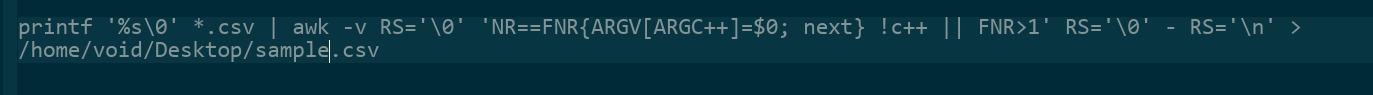
\includegraphics[scale=0.42]{chapter2}
\end{center}
\end{figure}
\end{itemize}
\item Scraped the following information for 17,102 stations:
\begin{itemize}
\item Latitude
\item Longitude
\item Number of Checkins
\item Address (attached to google maps link)
\item Station Information (availability at time of scrape, type of charger, name of network (i.e., ChargePoint), number of stations - this is in one single string, would need to be parsed)
\item Location ID (already known)
\end{itemize}
\item Scraped 75,064 reviews for 2,248 stations, with the following information parsed
\begin{itemize}
\item Url
\item Problem with charger -- (i.e., broken hardware, could not activate, blocked by vehicle)
\item kilowatts used when charging
\item connector
\item usernames
\item user's vehicle
\item date when charging
\item comment made by user
\end{itemize}
\item Labeled all location URLs at time of scrape (473,693), but as of 5/12/2025, looks like there are now 474,097 stations
\begin{itemize}
\item Now, you can filter by state, for example consider the following location name:
\begin{itemize}
\item "Barberino Nissan Parts | Wallingford, CT | EV Station"
\item Name states that this is in Connecticut, so you could write a code that filters for CT with ", CT |"
\end{itemize}
\end{itemize}
\item You can get the full reviews from the embeddable map from Plugshare, but they are anonymized and the map is cumbersome to operate. Link is \href{https://developer.plugshare.com/embed.html}{here} for further investigation.
\item Next things to do:
\begin{itemize}
\item Running in parallel without IP address getting banned, and moving to Yale's HPC - have tested on HPC but need the libnss library in order for google chrome to run headless
\item Parsing out availability information using tidyverse and adding date of scrape,
\item "J-1772 4 Plugs 6.48 kW 2 Stationscheck\_circle3 Availableaccount\_circle1 In Useremove\_circle0 UnavailableChargePoint Non-networked"
\item filtering out international charging stations completely and creating a comprehensive list for each state
\end{itemize}
\end{itemize}

\end{document}